\documentclass[a4paper,11pt,oneside]{article}
\usepackage[utf8]{inputenc}
\usepackage[french,english]{babel}
\usepackage{ae,aecompl,aeguill}
\usepackage[left=3cm,right=3cm,top=3cm,bottom=4cm]{geometry}
\usepackage{graphicx}
\usepackage[T1]{fontenc}

\newcommand{\file}[1]{\textsf{#1}}
\newcommand{\url}[1]{\selectlanguage{english}\file{#1}\selectlanguage{french}}


\begin{document}
%\sloppy
\selectlanguage{french}

\begin{titlepage}

{\noindent\small
\begin{tabular}[t t]{@{} p{.5 \textwidth} @{} p{.5 \textwidth} @{}}
  \begin{minipage}[t]{.5 \textwidth}
    Benjamin~\textsc{Gaillard}\\
    Nicolas~\textsc{Riegel}
  \end{minipage}
  &
  \begin{minipage}[t]{.5 \textwidth}
    \begin{flushright}
      IUP GMI 2\ieme{} année\\
      2004/2005
    \end{flushright}
  \end{minipage}
\end{tabular}
}
\vspace{5cm}

\begin{center}
\sc\huge
\scalebox{1.3}{Projet de Programmation}\\[1cm]
\scalebox{1.3}{Orientée Objet :}\\[2cm]
{\Huge \scalebox{1.3}{BoxLand}}\\[1cm]
\rule[5pt]{.5\textwidth}{2pt}\\[2cm]
\scalebox{1.3}{Rapport}
\end{center}

\end{titlepage}


\tableofcontents


\newpage
\section{Introduction}

\subsection{Rappel du sujet}
Le but est d'implémenter un jeu graphique simple (utilisant gtkmm).
Les critères suivants seront notés, par ordre d'importance décroissante :
\begin{itemize}
	\item La qualité de la conception orientée objet.
	\item La qualité des commentaires. Les commentaires doivent expliquer le sens de chaque bloc de code, ils sont
	adressés à un lecteur qui essaie de comprendre votre programme. Les commentaires ne doivent pas répéter ce qu'il
	y a dans le code. Les commentaires ne doivent pas expliquer les éléments syntaxiques, mais plutôt la sémantique.
	\item La lisibilité du code : choix des noms de classes, des membres, des variables et des fichiers. Votre programme
	doit être proprement divisé en plusieurs fichiers. Faites attention à l'indentation.
	\item Le résultat et les fonctionnalités du programme.
\end{itemize}
\begin{description}
	\item[Avertissement : ]La qualité prime sur la quantité. Un programme court mais bien organisé et bien commenté sera
	mieux noté qu'un gros programme mal conçu et incompréhensible.
\end{description}

\subsection{Choix du jeu : BoxLand}
Nous avons choisi de réaliser un jeu de type Boxworld. Le principe est assez simple : vous devez remettre des caisses à leur place,
mais vous ne pouvez pousser qu'une caisse à la fois.
La subtilité du jeu réside dans la réflexion. En effet, plus vous augmentez dans les niveaux, plus ce sera dur car les caisses sont
placées de telle sorte à ce que la solution soit de moins en moins facile à trouver. Voici un petit exemple du niveau 3 :
\begin{center}
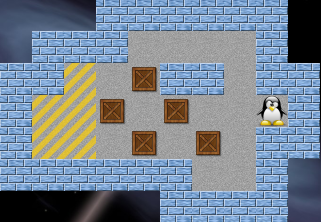
\includegraphics[keepaspectratio=true]{capture}
\end{center}
Vous noterez bien que tous les niveaux sont faisables, il n'y a pas de niveau piège.

\subsection{Comment jouer ?}
Ce jeu est conçu pour les plates formes Unix et Gtkmm doit être installé. Nous avons travaillé avec gtkm2.4, il peut y avoir des
problèmes de compatibilité avec d'autres versions. Si vous n'avez pas Gtkmm, vous pouvez vous le procurer sur le site : \\
\url{http://www.gtkmm.org/} \\
Pour lancer le jeu il vous suffit de vous rendre dans le répertoire et de tapez les commandes suivantes :
\begin{verbatim}
make
./boxland
\end{verbatim}
Dans ce programme, vous pourrez utiliser les touches suivantes :
\begin{description}
	\item[Echap ou Q :] Dans le menu, quitte le jeu. Dans le jeu, quitte le niveau et revient au menu.
	\item[Haut,Bas,Gauche,Droite ou 8,2,4,6 :] Vous pouvez utilisez les flèches ou le pavé numérique pour vous déplacer, aussi
	bien dans le menu que pendant le jeu.
	\item[Entrée ou Espace :] Dans le menu, sert à lancer le jeu avec le niveau sélectionné.
	\item[Espace ou P :] Dans le jeu, met en pause.
	\item[Backspace ou U :] Dans le jeu, annule votre dernier déplacement.
	\item[R :] Dans le jeu, recommence le niveau en cours.
\end{description}


\newpage
\section{Les niveaux}

Les niveaux sont stockés dans des fichiers textes dans le répertoire \file{levels/}. Voici à quoi ressemble un de ces fichier :
\begin{verbatim}
#########.
#   ##  #.
# # % % #.
#  *X#  #.
## #X$X##.
##%###*###
#        #
#   ## # #
######   #
.....#####
\end{verbatim}%$ emacs...
Vous constatez donc que ces niveaux sont lisibles et ne sont pas des fichiers compliqués. Cela permet de rajouter facilement des
niveaux que vous aurez créé vous-même ou que vous aurez trouvé sur internet. Seuls quelques symboles sont à connaitre. En voici
la liste :
\begin{itemize}
	\item `\verb*|#|' (dièse): représente un mur ;
	\item `\verb*| |' (espace) : représente le sol ;
	\item `\verb*|X|' : représente une case d'arrivée pour les caisses ;
	\item `\verb*|.|' (point) : permet de mettre des décallages hors du niveau (donc rien n'est affiché à la place du point) ;
	\item `\verb*|$|' (dollar) : correspond au point de départ du personnage ;
	\item `\verb*|%|' (pourcent) : correspond au point de départ d'une caisse ;
	\item `\verb*|*|' (astérisque) : correspond au point de départ d'une caisse qui est déjà sur une case d'arrivée.
\end{itemize}
Il y a quand même quelques contraintes de faisabilité. Par exemple vous ne pouvez pas mettre un nombre de caisses supérieur au nombre
de cases d'arrivées. De plus, il faut que votre niveau soit réellement faisable. Or le programme n'est pas fait pour tester ça, donc
c'est à vous de vérifier cela. L'occasion est bonne pour vous rappeler que tous les niveaux fournis avec le jeu sont faisables. :)


\newpage
\section{Structure du programme}

\subsection{Diagramme des classes}
\begin{center}
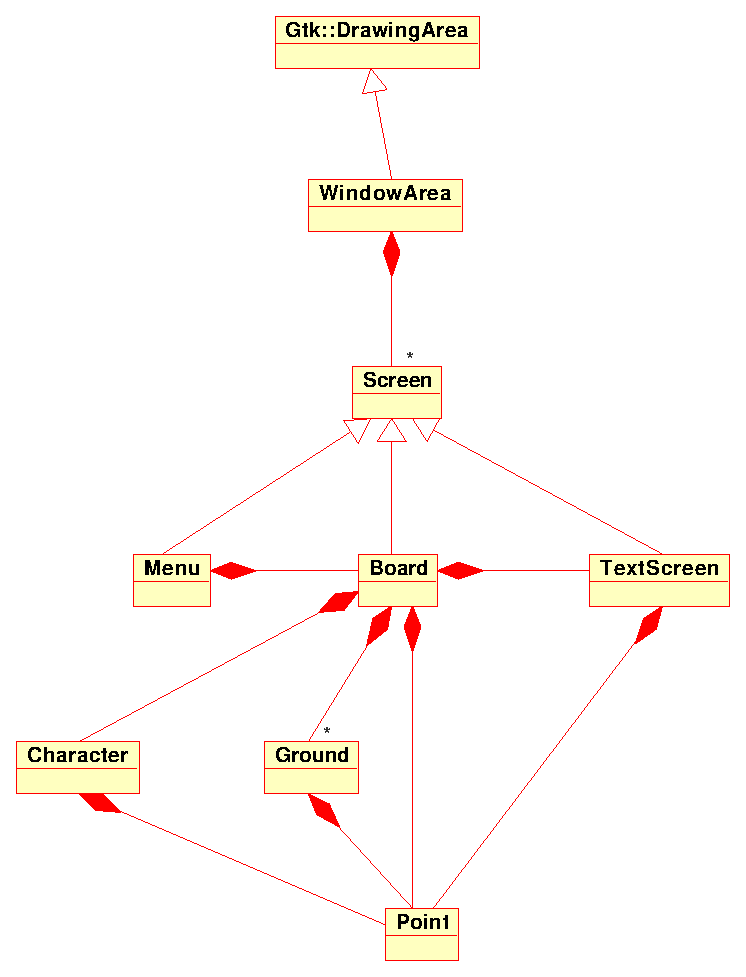
\includegraphics[height=\textwidth,keepaspectratio=true]{diagramme}
\end{center}

\subsection{Classe Point}
Cette classe permet de stocker des coordonnées dans le plan. Elle contient 3 constructeurs, 2 fonctions pour changer les valeurs des
coordonnées, et surdéfinit les opérateurs +,-,+=,-=,*=,== et !=. Les valeurs des 2 coordonnées sont stockées dans x et y.

\subsection{Classe Character}
Cette classe sert à l'affichage et au déplacement du personnage et éventuellement d'une caisse qu'il déplace, et cela grâce aux
fonctions :
\begin{itemize}
\item\verb|void Draw();|
\item\verb|bool Move(Direction dir);|
\item\verb|bool Timeout();|
\end{itemize}
La dernière de ces 3 est utilisée pour l'animation du personnage. En effet le personnage ne se déplace pas d'un coup, mais
progressivement. Vous pouvez règler la vitesse du déplacement dans le fichier \file{config.h}.
Dans cette classe est aussi stockée la position du personnage.
C'est aussi dans cette classe que va être implémentée la fonction qui annule le dernier déplacement du personnage.

\subsection{Classe Ground}
Cette classe gère tout ce qui est case. Elle permet de dessiner les cases (mur, sol, case d'arrivée de caisse, etc...) ainsi que de faire
des tests sur le genre de case, pour pouvoir vérifier par exemple si la caisse est sur une case d'arrivée :
\begin{itemize}
\item\verb|void Draw(const Board &board) const;|
\item\verb|bool IsWalkable() const;|
\item\verb|bool IsEnd() const;|
\end{itemize}

\subsection{Classe Screen}
Cette classe est une classe abstraite qui sert à définir les fonctions que devront implémenter les classes dérivées et qui
s'occupe aussi de gérer une fonction de base :
\begin{itemize}
\item\verb|void SetWindowArea(WindowArea *warea);|
\end{itemize}
Cette fonction est utile pour les classes dérivées, qui n'auront rien de spécial à faire quand elle dériveront,
et auront directement accès aux variables \verb|area|, \verb|window|, \verb|gc| et \verb|cm|, qui seront correctement initialisées.
Les 2 fonctions suivantes servent au changement d'écran :
\begin{itemize}
\item\verb|void Switch(Screen *screen) const { if (area) area->Switch(screen); }|
\item\verb|void Return()               const { if (area) area->Return();       }|
\end{itemize}
Les fonctions que devront implémenter les classes dérivées sont :
\begin{description}
	\item[virtual void OnInit();] actions à effectuer lors de la création de l'écran
	\item[virtual void OnEnter();] actions à effectuer lorsqu'on va utiliser cet écran
	\item[virtual void OnLeave();] actions à effectuer lorsqu'on quitte l'écran
	\item[virtual void OnDraw();] actions à effectuer lorsqu'on redessine l'écran
	\item[virtual void OnKeyPressed(unsigned int key);] actions à effectuer lorsqu'on appuie sur une touche
\end{description}
De plus cette classe permet aux fonctions dérivées de dessiner différents éléments : images, textes, rectangles, et de modifier les couleurs.
En effet les fonctions de dessin sont dans la classe \verb|WindowArea| qui est mise comme classe amie.

\subsection{Classe WindowArea}
Cette classe dérive de la classe \verb|Gtk::DrawingArea|. Elle s'occupe d'appeler les fonctions de gestion du clavier et
d'affichage avec les fonctions :
\begin{itemize}
\item\verb|virtual void on_realize();|
\item\verb|virtual bool on_expose_event(GdkEventExpose *event);|
\item\verb|virtual bool on_key_press_event(GdkEventKey *event);|
\end{itemize}
Elle permet de changer facilement et rapidement d'une classe \verb|Screen| à une autre sans avoir à se soucier des
ressources graphiques. C'est en quelque sorte un gestionnaire d'écrans. Pour cela elle utilise les fonctions suivantes :
\begin{itemize}
\item\verb|void Switch(Screen *screen);|
\item\verb|void Return();|
\end{itemize}
Cette classe stocke aussi tous les écrans grâce à la classe :\\
\verb|vector| : \verb|std::vector<Screen *> screens;|.\\
De plus c'est dans cette classe que sont les fonctions de dessins d'images, de textes et de rectangles.

\subsection{Classe TextScreen}
Cette classe dérive de la classe \verb|Screen|. C'est une classe simple qui va se charger d'afficher une image au centre de l'écran,
uniquement ça. Elle va aussi transmettre les événements provenant du clavier à la classe Screen qui l'a créée. Lorsque l'affichage de
l'écran est demandé, \verb|TextScreen| va d'abord appeler la méthode d'affichage de la classe \og appelante\fg{} puis afficher son image.
Cela permet d'afficher une image par transparence sur l'écran précédent. Elle est utilisée au moyen des fonctions :
\begin{itemize}
\item\verb|void SetImage(...);| pour choisir une image à afficher ;
\item\verb|void Terminate();  | pour retourner à l'écran précédent.
\end{itemize}
L'affichage est déclenché en utilisant la méthode \verb|Switch()| de la classe \verb|WindowAre|a ou \verb|Screen|.

\subsection{Classe Board}
Cette classe hérite de la classe \verb|Screen| pour pouvoir afficher dans la fenêtre graphique et redéfinit donc les différentes fonctions
dont elle hérite. C'est la classe qui va gérer l'affichage du jeu, le moteur de jeu et tout ce qui concerne le jeu en lui-même.
Par exemple, il y a la fonction
\begin{itemize}
\item\verb|bool LoadMap(const std::string &filename);|
\end{itemize}
qui va charger le niveau, et d'autres fonctions pour l'affichage des images, du personnage, des caisses et des informations :
\begin{itemize}
\item\verb|void DrawBoxImage(...)|
\item\verb|void DrawBox(const Point &pos) const;|
\item\verb|void DrawCharacter() const;|
\item\verb|void DrawInformations();|
\end{itemize}
Enfin il y a deux tableaux, un pour stocker l'emplacement des murs, sols et cases d'arrivées :
\begin{itemize}
\item\verb|Ground map[MAX_MAP_HEIGHT][MAX_MAP_WIDTH];|
\end{itemize}
et l'autre pour stocker l'emplacement des caisses :
\begin{itemize}
\item\verb|bool isBox[MAX_MAP_HEIGHT][MAX_MAP_WIDTH];|
\end{itemize}
Cette classe sert aussi à stocker les images du jeu :
\begin{itemize}
\item\verb|Glib::RefPtr<Gdk::Pixbuf> images[IMG_COUNT];|
\end{itemize}
qu'elle va charger grâce à la fonction
\begin{itemize}
\item\verb|void LoadImages();|
\end{itemize}
Enfin, la dernière fonction de cette classe et de stocker le temps écoulé, le nombre de mouvements effectués, le nombre de caisses
qui ne sont pas encore sur une case d'arrivée et le personnage :
\begin{itemize}
\item\verb|unsigned int time;|
\item\verb|unsigned int moves;|
\item\verb|unsigned int remain;|
\item\verb|Character charact;|
\end{itemize}
Des fonctions sont disponibles pour récupérer ces valeurs et même pour en modifier certaines.

\subsection{Classe Menu}
Cette classe aussi hérite de \verb|Screen| pour pouvoir afficher tout ce qui concerne le menu, notament le choix du niveau. Elle
redéfinit donc aussi les différents fonctions dont elle hérite. C'est aussi elle qui va créer les objets \verb|Board| alors que
l'objet \verb|Menu| est lui créé dans le \verb|main|. La classe \verb|Menu| est chargée de chercher les noms des différents niveaux
avec la fonction
\begin{itemize}
\item\verb|bool LoadLevels();|
\end{itemize}
Elle stocke les noms dans un tableau grâce à la classe \verb|vector| :
\begin{itemize}
\item\verb|std::vector<std::string> levels;|
\end{itemize}
C'est aussi elle qui vérifie s'il y a un niveau suivant :
\begin{itemize}
\item\verb|bool NextLevel();|
\end{itemize}


\newpage
\section{Choix d'implémentation}

La plupart des classes incluent certaines méthodes très simples. Elles ont été implémentées dans la déclaration de la classe directement,
afin qu'elles soient insérées de façon \emph{inline} dans le code qui les appelle. Ces méthodes ne comportent en général qu'une seule
instruction, parfois deux, mais restent très simple et écrites sur une seule ligne. À partir du moment où leur implémentation nécessite
plus d'instructions, ou que ces méthodes sont virtuelles, elles sont écrites comme les autres dans les fichiers d'implémentation (.cpp).

Il est intéressant de noter que toutes les classes comportent le maximum de leurs éléments dans des sections protégées (\verb|private| et
\verb|protected|). Uniquement les méthodes ayant vraiment besoin d'être accédées depuis d'autres classes sont présentes en tant que
méthodes publiques, ou les données de classes très simple (classe \verb|Point|). Certaines méthodes qui auraient du être publiques mais
qui ne sont destinées à être utilisées que par une seule autre classe sont dans une section \verb|private|, et la classe associée est
déclarée en tant que classe amie.

La classe \verb|Point| n'est implémentée qu'en un seul fichier d'en-tête (.h), du fait de sa très grande simplicité. Toutes les autres
classes sont séparées en deux fichiers : un fichier d'implémentation (.cpp) et un fichier d'en-tête déclarant la classe (.h).


\newpage
\section{Conclusion}

Ce projet nous a permis d'approfondir nos connaissances dans le langage C++ acquises lors des cours, TDs et TPs.
De plus il nous a fait découvrir la notion d'interface graphique à travers Gtkmm. Même s'il se raconte ici ou là que Gtkmm n'est pas l'outil
idéal pour les jeux, nous avons réussi à nous adapter. Concernant le choix du jeu, nous avons préféré choisir un petit jeu sympa et sur
lequel on y passe des heures et des heures plutôt qu'un gros jeu avec des millions d'options et de possibilités. Si vous arrivez à terminer
tous les niveaux facilement, c'est que vous êtes vraiment doué. :-)


\end{document}
